\documentclass{standalone}
\usepackage{tikz}
\usepackage{customdice}
\usepackage{amsmath}

\newcommand{\addictiondice}[4]{\node at (#1,#2) {\Huge\sffamily\textdice[lightgray,black]{#3\(_\text{\large #4}\)}};}

\begin{document}\setdicefacesize{2}
    
    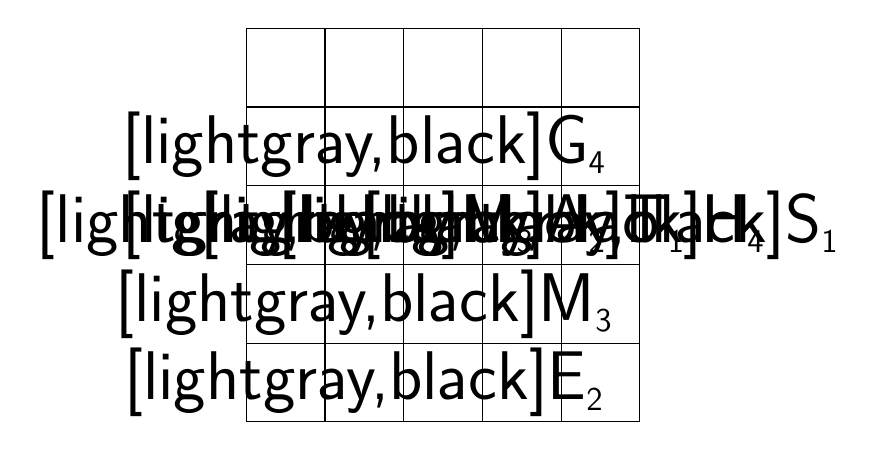
\begin{tikzpicture}
        \begin{scope}[shift={(-1.5,-0.5)}]
            \draw (0,0) grid (5,5);
        \end{scope}
        
        \addictiondice{-1}{2}{M}{3}
        \addictiondice{1}{2}{T}{1}
        \addictiondice{2}{2}{H}{4}
        \addictiondice{3}{2}{S}{1}
        
        \addictiondice{0}{3}{G}{4}
        \addictiondice{0}{2}{A}{2}
        \addictiondice{0}{1}{M}{3}
        \addictiondice{0}{0}{E}{2}
    \end{tikzpicture}
    
\end{document}

